\documentclass{report}

%%%%%%%%%%%%%%%%%%%%%%%%%% Practice info %%%%%%%%%%%%%%%%%%%%%%%%%%
\Subject {Системи штучного інтелекту}
\DocTitle{Обчислення в обчислювальних графах: зворотне поширення помилки}
\ReportType{Семінар}

%----------------------------------------------------
%	  Персональна інформація виконавця завдання
%----------------------------------------------------
\Done{Виконав:}  % Поставте правильне закінчення


\Surname{Бардін}  		% Вкажіть своє прізвище
\Name{Владислав}		% та ім'я
\Group {ІМ-42мп}     		% група в якій навчаєтесь
\YearOfStudying {5}		% курс навчання


%%%%%%%%%%%%%%%%%%%%%%%%%%%%%%%%%%%%%%%% ПОЧАТОК ЗВІТУ %%%%%%%%%%%%%%%%%%%%%%%%%%%%%%%%%%%%%%%%
\startDocument

\newpage
\section{\doctitle}

Сьогодні нейронні мережі — це не просто наукова теорія, а реальний інструмент, який активно використовується в повсякденому житті. Вони допомагають розпізнавати обличчя на фото, рекомендувати фільми, ставити медичні діагнози та навіть передбачати ринкові зміни. Але щоб нейронна мережа працювала правильно, її потрібно навчити. Для цього важливо оптимізувати її параметри. Тут на допомогу приходить алгоритм зворотного поширення помилки, або backpropagation.

Цей алгоритм став справжнім проривом у машинному навчанні. Завдяки йому вдалося навчити складні багатошарові нейронні мережі, які раніше вважалися практично неможливими для використання. Backpropagation дозволяє мережі поступово зменшувати свої помилки і покращувати результати, використовуючи досить просту математику.

\subsection{Історія алгоритму}
Ідеї, які лежать в основі алгоритму backpropagation, з’явилися ще в 1974 році~\cite{Werbos1974}. Пол Вербос у своїй роботі запропонував спосіб обчислення градієнтів у складних моделях. Проте справжню популярність алгоритм здобув завдяки статті Джефрі Гінтона, Девіда Румельхарта і Рональда Вільямса у 1986 році~\cite{Hinton1986}. Вони змогли детально пояснити, як алгоритм можна застосовувати для навчання багатошарових мереж. Ця стаття стала переломним моментом у дослідженні нейронних мереж. Вчені довели, що такі мережі можуть ефективно працювати, якщо правильно оновлювати їх параметри на основі похибок.

\subsection{Як працює алгоритм}
Головна ідея backpropagation дуже проста. Мережа спочатку обчислює результат (це називається forward pass), а потім порівнює його з правильним значенням. Якщо є помилка, алгоритм визначає, як потрібно змінити кожен параметр, щоб зменшити цю помилку (це називається backward pass).

Forward pass допомагає мережі зробити прогноз. Наприклад, у задачі розпізнавання цифр на зображеннях, мережа спробує вгадати, яка цифра намальована. Потім backward pass обчислює, наскільки кожен параметр вплинув на помилку. Ця інформація використовується, щоб трохи змінити параметри і зробити мережу точнішою.

\subsection{Чому алгоритм важливий}
Backpropagation дозволяє нейронним мережам навчатися автоматично. Це зробило їх доступними для вирішення складних задач у багатьох галузях. Наприклад, алгоритм допомагає:
- Розпізнавати обличчя, текст або об’єкти на фото.
- Аналізувати емоції у текстах або перекладати їх іншими мовами.
- Пропонувати фільми чи товари, які можуть вас зацікавити.

Без цього алгоритму сучасні системи штучного інтелекту не могли б бути такими ефективними. Він забезпечує їхню здатність швидко адаптуватися до нових даних і став основою для багатьох технологій.

\newpage
\section{Поняття обчислювальних графів}
Алгоритм зворотного поширення помилки є основою навчання нейронних мереж. Його ефективність значною мірою базується на використанні обчислювальних графів. Ці графи забезпечують зручний та структурований підхід до представлення обчислень, що робить алгоритм потужним і універсальним.

\subsection{Обчислювальний граф?}
Обчислювальний граф (англ. computational graph) — це математична модель, яка представляє обчислення у вигляді орієнтованого графа. У цьому графі:
\begin{itemize}
    \item Вузли відповідають операціям або функціям (наприклад, додавання, множення, застосування активаційної функції).
    \item Ребра показують передачу результатів між операціями.
\end{itemize}

Ця структура дозволяє розбивати складні обчислення на простіші кроки, які можна виконувати послідовно або паралельно. Завдяки цьому обчислювальні графи є основою для автоматичного обчислення градієнтів за допомогою правила ланцюгового диференціювання.

\subsection{Основні переваги обчислювальних графів}
Ключовою особливістю обчислювального графа є можливість поділу обчислень на послідовні кроки. Це надає низку переваг:
\begin{itemize}
    \item зручна візуалізація всього ланцюга обчислень;
    \item автоматизація процесу диференціювання;
    \item підтримка паралельного виконання незалежних кроків, що підвищує ефективність.
\end{itemize}

Завдяки цьому можна легко проаналізувати, яким чином початкові вхідні змінні впливають на кінцевий результат, а також кроки, що не залежать один від одного, можуть виконуватися паралельно, що робить обчислення швидшими та ефективнішими.

\subsection{Приклад обчислювального графа}

Як приклад розглянемо просту функцію з двома змінними x та y:
\begin{equation}
	f(x,y)=(x+y)×y
\end{equation}

\begin{figure}[hbt!]
  \center
  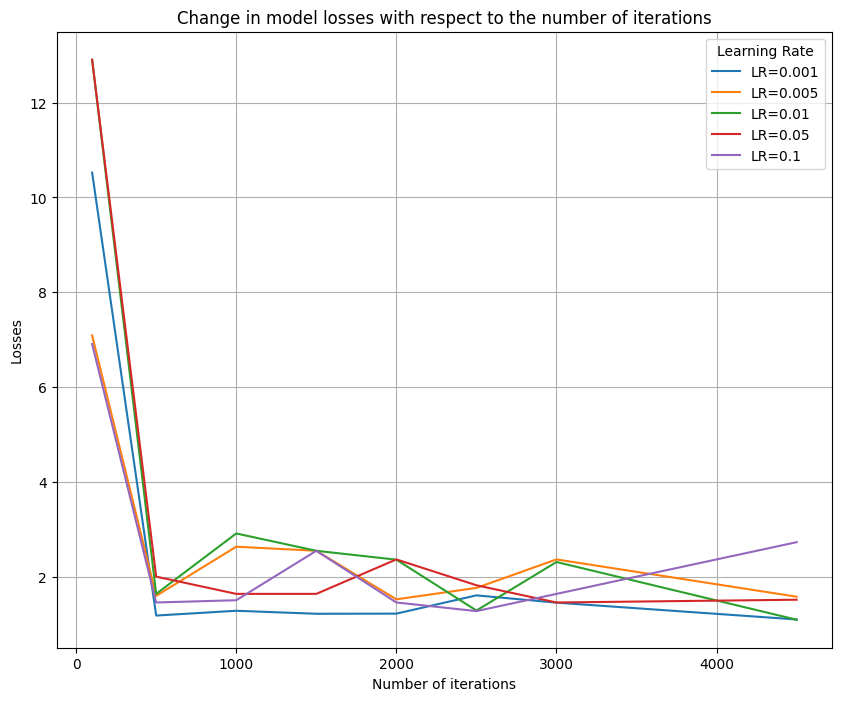
\includegraphics[scale=0.5]{fig1}
  \caption{Обчислювальний граф для функції}
   \label{im:fig1}
\end{figure}

Обчислення цього графу можна подати у вигляді вузла А, який отримує 2 вхідні параметри x та y, та виконує операцію додавання x+y. Та вузла Б, який отримує як вхідні параметри y та результат виконання вузла А (x+y) виконуючи множення ((x+y)×y).

Сформувавши таку схему нею можна зробити 2 проходи, у прямому (forward pass) та зворотному напрямку (backward pass). Прямий обхід застосовується для обчислення кінцевого значення функції, а зворотній для обчислення градієнтів відносно змінних x та y.

\subsection{Значення для нейронних мереж}
Завдяки такому підходу у складних нейронних мережах з багатьма шарами і безліччю параметрів ми можемо системно структурувати процес. Замість монолітного обчислення маємо послідовну (або й паралельну) сукупність вузлів і ребер, де кожна операція виконується у чітко визначеному порядку.

Таким чином, обчислювальні графи є фундаментом для реалізації алгоритму зворотного поширення помилки, оскільки саме завдяки чіткій структурі вузлів і ребер можна коректно та швидко знайти градієнти кожного параметра, впливаючи на точність і швидкість навчання штучних нейронних мереж.

\newpage
\section{Загальна ідея алгоритму зворотного поширення помилки}

Зворотне поширення помилки — це ефективний метод оптимізації, що використовується для корекції вагових параметрів нейронної мережі з метою мінімізації функції втрат. Алгоритм ґрунтується на правилі ланцюгового диференціювання, що дозволяє обчислювати похідні (градієнти) функції втрат по кожному параметру мережі.

Для виконання прямого проходу вхідні дані подаються на вхід мережі, проходять через усі шари з відповідними функціями активації, і на виході отримується прогноз. Після цього обчислюється значення функції помилки, наприклад, сума квадратів різниць між передбаченими та реальними виходами, або крос-ентропія. Обчислене значення функції помилки використовується для руху у зворотному напрямку, послідовно обчислюючи частинні похідні відносно кожної ваги. Таким чином ми отримуємо інформацію про те, як змінити кожен параметр мережі, щоб зменшити загальну помилку.

У загальному випадку, якщо вихідна помилка позначається як E, а проміжна змінна як z, то похідну dE/dz можна обчислити через інші змінні u,v… згідно з правилом ланцюга:
\begin{equation}
	\frac{dE}{dz} = \frac{dE}{du} \cdot \frac{du}{dv} \cdot \dots \cdot \frac{dw}{dz}
\end{equation}
У контексті нейронної мережі кожен “ланцюг” відповідає шляху в обчислювальному графі від параметра до підсумкової функції помилки.
Після обчислення градієнтів алгоритм зворотного поширення помилки зазвичай застосовується у поєднанні з методом градієнтного спуску, який оновлює кожну вагу $W_{ij}$ у напрямку протилежному до градієнта:
\begin{equation}
	W_{ij} \leftarrow W_{ij} - \eta \cdot \frac{dE}{dW_{ij}}
\end{equation}

де $\eta$ – швидкість навчання.
 
Це дозволяє послідовно зменшувати значення функції помилки на кожній ітерації, поки мережа не досягне прийнятної точності.

Загалом, алгоритм зворотного поширення помилки — це “серце” навчання більшості глибинних нейронних мереж. Він дає змогу поєднати переваги обчислювальних 
графів з математикою ланцюгового диференціювання, що в підсумку забезпечує ефективне й точне оновлення параметрів моделі.

Для прикладу розглянемо просту нейронну мережу з одним прихованим шаром.
Прямий прохід на кожному шарі обчислюється як:
\begin{equation}
	z^{(l)} = W^{(l)} a^{(l-1)} + b^{(l)}
\end{equation}

\begin{equation}
	a^{(l)} = \sigma(z^{(l)})
\end{equation}

де:
\begin{itemize}
	\item $z^{(l)}$ – вхідні значення нейронів на шарі $l$,
	\item $W^{(l)} i b^{(l)}$ – ваги та зсуви,
	\item $\sigma$ – функція активації,
	\item $a^{(l-1)}$ – вихід нейронів на шарі $l$.
\end{itemize}

обислення функції втрат відбувається за формулою:
\begin{equation}
	\mathcal{L} = \frac{1}{2} \sum_{i} \left( y_i - \hat{y}_i \right)^2
\end{equation}

де:
\begin{itemize}
	\item $y_i$ – очікуваний результат,
	\item $\hat{y}_i$ – передбачення моделі.
\end{itemize}

Зворотній прохід обчислюється за формулами:

Градієнти обчислюються, починаючи з вихідного шару, за допомогою правила ланцюгового диференціювання:
\begin{equation}
	\delta^{(L)} = \frac{\partial \mathcal{L}}{\partial z^{(L)}} = \left( \hat{y} - y \right) \cdot \sigma'(z^{(L)})
\end{equation}

для попередніх шарів використовується:
\begin{equation}
	\delta^{(l)} = \left( W^{(l+1)} \right)^T \delta^{(l+1)} \cdot \sigma'(z^{(l)})
\end{equation}

Оновлення ваг здійснюється за правилом граждієнтного спуску:
\begin{equation}
	W^{(l)} := W^{(l)} - \eta \frac{\partial \mathcal{L}}{\partial W^{(l)}}
\end{equation}

\begin{equation}
	b^{(l)} := b^{(l)} - \eta \frac{\partial \mathcal{L}}{\partial b^{(l)}}
\end{equation}

де $\eta$ – швидкість навчання.

Наприклад, розглянемо функцію з двома змінними $f(x, y) = (x + y)^2$.
\begin{figure}[hbt!]
  \center
  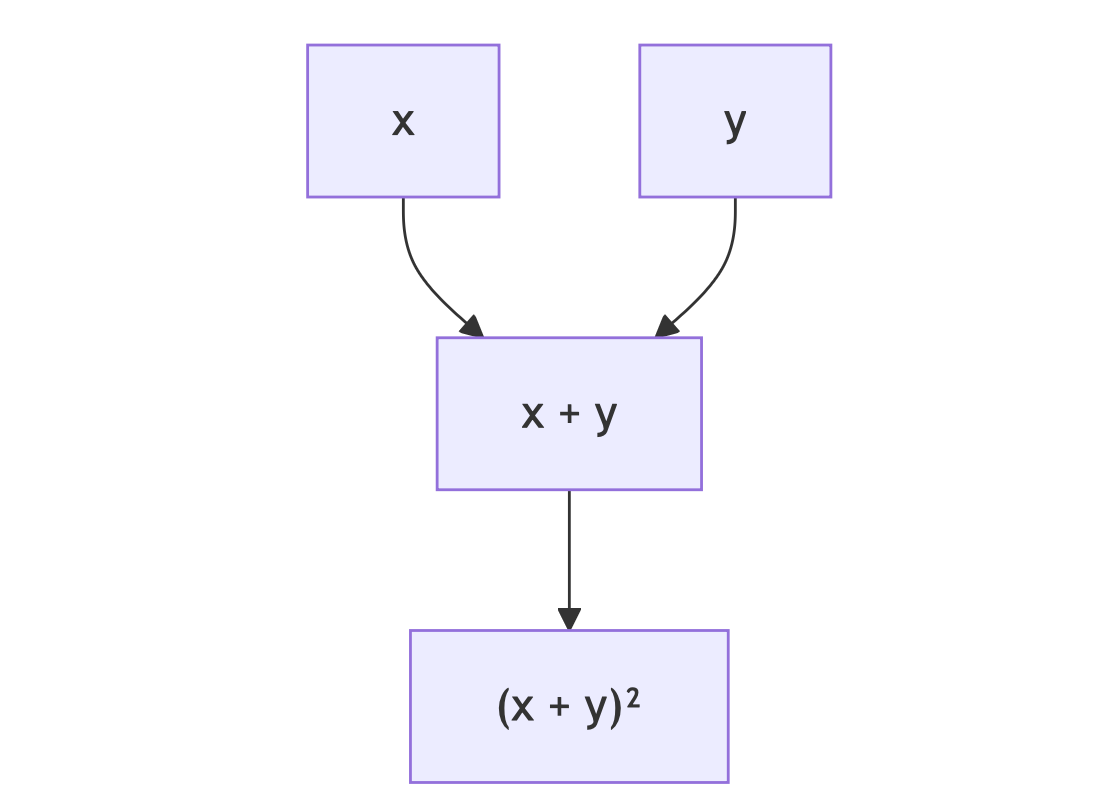
\includegraphics[scale=0.3]{fig2}
  \caption{Обчислювальний граф для функції}
   \label{im:fig2}
\end{figure}

Прямий прохід:
Вхідні дані $x = 2, y = 3$, тоді $f(x, y) = (x + y)^2 = (2 + 3)^2 = 25$.

\begin{figure}[hbt!]
  \center
  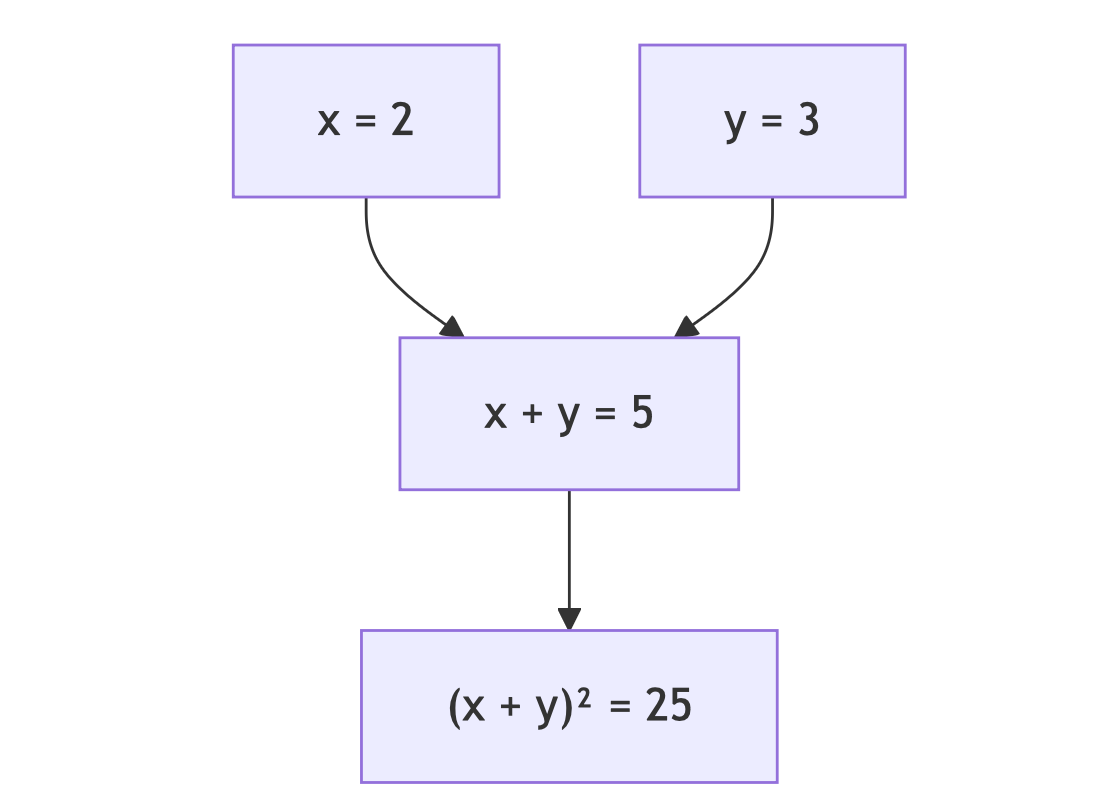
\includegraphics[scale=0.3]{fig3}
  \caption{Схема прямого проходу з обчисленням проміжних значень}
   \label{im:fig3}
\end{figure}

Зворотній прохід:
\begin{figure}[hbt!]
  \center
  \includegraphics{•}
  [scale=0.3]{fig4}
  \caption{Схема обчислення градієнтів при зворотньому проході}
   \label{im:fig4}
\end{figure}

Для похідних використовуємо
\begin{equation}
	\frac{\partial f}{\partial x} = 2(x + y), \quad \frac{\partial f}{\partial y} = 2(x + y)
\end{equation}

Підставляючи $x$ та $y$ отримаємо
\begin{equation}
	\frac{\partial f}{\partial x} = 2(2 + 3) = 10, \quad \frac{\partial f}{\partial y} = 2(2 + 3) = 10
\end{equation}

\newpage
\section{Практичне застосування backpropagation}

Алгоритм зворотного поширення помилки (backpropagation) є фундаментальним елементом процесу навчання нейронних мереж. Завдяки своїй ефективності він став основою для багатьох практичних застосувань у різних сферах. Розглянемо детальніше, як саме алгоритм використовується і чому його застосування є доцільним.

\subsection{Розпізнавання образів}
Розпізнавання образів є однією з ключових задач машинного навчання. Алгоритм backpropagation використовується для навчання моделей класифікації зображень, таких як багатошарові персептрони (MLP) або згорткові нейронні мережі (CNN).

\begin{itemize}
    \item Під час forward pass зображення, представлене у вигляді вектору пікселів, проходить через шари нейронної мережі, де кожен шар виконує лінійні перетворення і функції активації.
    \item На виході мережі отримується набір ймовірностей, що відповідають кожному класу (наприклад, цифрам 0-9 для набору даних MNIST).
    \item У backward pass алгоритм backpropagation обчислює градієнти функції втрат (наприклад, крос-ентропії) за кожною вагою мережі, використовуючи правило ланцюгового диференціювання.
    \item Ваги оновлюються за допомогою градієнтного спуску, щоб зменшити помилку між передбаченим і реальним класом.
\end{itemize}

Backpropagation дозволяє систематично знижувати помилку, адаптуючи ваги мережі до складних закономірностей у зображеннях. У результаті модель досягає точності понад 98\% на MNIST, що робить її практично застосовною для автоматизації завдань розпізнавання.

\subsection{Обробка природної мови}
У задачах обробки природної мови (NLP), таких як класифікація тексту, машинний переклад або аналіз тональності, backpropagation використовується для оптимізації моделей, зокрема рекурентних нейронних мереж (RNN) та трансформерів.

\begin{itemize}
    \item Вхідний текст перетворюється у числові векторні уявлення (word embeddings), які подаються на вхід нейронної мережі.
    \item Під час forward pass мережа аналізує послідовності слів, враховуючи їхній контекст.
    \item У backward pass алгоритм backpropagation через час (backpropagation through time, BPTT) розраховує похідні для кожного стану RNN, дозволяючи оновлювати ваги, що відповідають за довгострокові залежності у тексті.
\end{itemize}

Алгоритм дозволяє враховувати контекст попередніх слів, що є критично важливим для аналізу послідовностей. Наприклад, у задачі класифікації відгуків модель може визначити емоційне забарвлення фраз, таких як "дуже хороший" або "абсолютно жахливий". Це забезпечує точність понад 90\%.

\subsection{Рекомендаційні системи}
Рекомендаційні системи використовують backpropagation для персоналізації рекомендацій на основі поведінки користувачів.

\begin{itemize}
    \item Кожного користувача і кожен товар система представляє у вигляді векторів (embeddings), які знаходяться у спільному просторовому представленні.
    \item Forward pass моделює ймовірність того, що користувач обере конкретний товар, на основі подібності між векторами користувача і товару.
    \item Backward pass використовується для мінімізації функції втрат, наприклад, кореня середньоквадратичної похибки (RMSE) між реальними і передбаченими рейтингами.
\end{itemize}

Backpropagation дозволяє постійно покращувати точність рекомендацій, адаптуючи систему до поведінки користувачів. Це сприяє збільшенню конверсії та покращенню взаємодії з платформою.

\subsection{Медицина та інші сфери}
Застосування алгоритму виходить далеко за межі вищезгаданих прикладів. Наприклад:
\begin{itemize}
    \item У медицині алгоритм використовується для аналізу зображень, таких як МРТ чи рентген, для виявлення патологій.
    \item У фінансах backpropagation допомагає прогнозувати ринкові тенденції, аналізуючи великі обсяги історичних даних.
    \item В ігровій індустрії алгоритм застосовується для навчання ігрових агентів, які здатні самостійно освоювати складні середовища.
\end{itemize}

\subsection{Підсумки}
Завдяки алгоритму backpropagation нейронні мережі здатні вирішувати задачі, які раніше здавалися неможливими. Його універсальність, ефективність і адаптивність роблять його незамінним інструментом у сучасному світі штучного інтелекту. Алгоритм забезпечує оптимізацію параметрів моделей, дозволяючи їм швидко і точно навчатися, що відкриває широкі можливості для інновацій у різних галузях.

\newpage
\section{ВИСНОВКИ}

Зворотне поширення помилки (backpropagation) є фундаментальним алгоритмом, який забезпечив прорив у сфері машинного навчання та глибинних нейронних мереж. Завдяки послідовному обчисленню градієнтів кожного параметра мережі та врахуванню усіх проміжних операцій в обчислювальному графі стало можливим навчати багатошарові моделі та отримувати вражаючі результати в різноманітних завданнях: від комп’ютерного зору до обробки природної мови і рекомендаційних систем.
У ході роботи над рефератом проаналізовано:
\begin{itemize}
	\item суть обчислювальних графів: їхня роль у структуризації всього процесу обчислень та наочне представлення операцій над даними;
	\item механізм та ідея backpropagation: від історичних витоків до конкретного алгоритмічного втілення; описано, як кожен параметр впливає на помилку на виході і як його оновити за правилом ланцюгового диференціювання.
\end{itemize}

Застосування зворотного поширення помилки разом із потужними засобами апаратного прискорення дає змогу обробляти величезні обсяги даних, будувати глибинні мережі й успішно розв’язувати складні прикладні завдання. Попри наявність альтернативних підходів, backpropagation залишається основою більшості сучасних рішень у галузі штучного інтелекту.

Backpropagation має перспективи подальших досліджень, що полягають у розробці покращених методів оптимізації, вивченні способів розв’язання проблеми зникаючих та вибухаючих градієнтів, а також у пошуку нових архітектур, здатних ще ефективніше використовувати потенціал зворотного поширення помилки. Це означає, що backpropagation та обчислювальні графи залишатимуться важливою складовою інструментарію машинного навчання у найближчому майбутньому.

\newpage

\begin{thebibliography}{99}

\bibitem{Goodfellow2016}
Goodfellow, I., Bengio, Y., and Courville, A. \textit{Deep Learning}. MIT Press, 2016.

\bibitem{Rumelhart1986}
Rumelhart, D. E., Hinton, G. E., and Williams, R. J. Learning representations by back-propagating errors. \textit{Nature}, 1986, Vol. 323, pp. 533-536.

\bibitem{Werbos1982}
Werbos, P. J. Applications of advances in nonlinear sensitivity analysis. \textit{System Modeling and Optimization}, Springer, Berlin, Heidelberg, 1982, pp. 762-770.

\bibitem{Nielsen2015}
Nielsen, M. \textit{Neural Networks and Deep Learning}. 2015. Retrieved from \url{http://neuralnetworksanddeeplearning.com}.

\bibitem{Bishop2006}
Bishop, C. M. \textit{Pattern Recognition and Machine Learning}. Springer, 2006.

\bibitem{Werbos1974}
Paul John Werbos. \textit{The Roots of Backpropagation: From Ordered Derivatives to Neural Networks and Political Forecasting}. Adaptive and Cognitive Dynamic Systems, 1974.

\bibitem{Hinton1986}
Geoffrey E. Hinton \textit{Learning Distributed Representations of Concepts}, 1986. Retrieved from \url{https://www.cs.toronto.edu/~hinton/absps/families.pdf}.

\end{thebibliography}
\end{document}
